For the numerical experiments, we first run the same experiments of \cite{buzna2007efficient} and reproduce \emph{figure 2} in original paper\cite{buzna2007efficient}. Then we compare the optimal strategy from our optimization with these six heuristic strategies.

\subsection{Reproducing Experiments of Original Paper}

In order to benchmark our model and codes, we first perform the same experiments as in the original paper\cite{buzna2007efficient} and reproduce \emph{figure 2} in \cite{buzna2007efficient}.


\begin{figure}	
	\centering
	\begin{subfigure}[t]{0.8\textwidth}
		\centering
		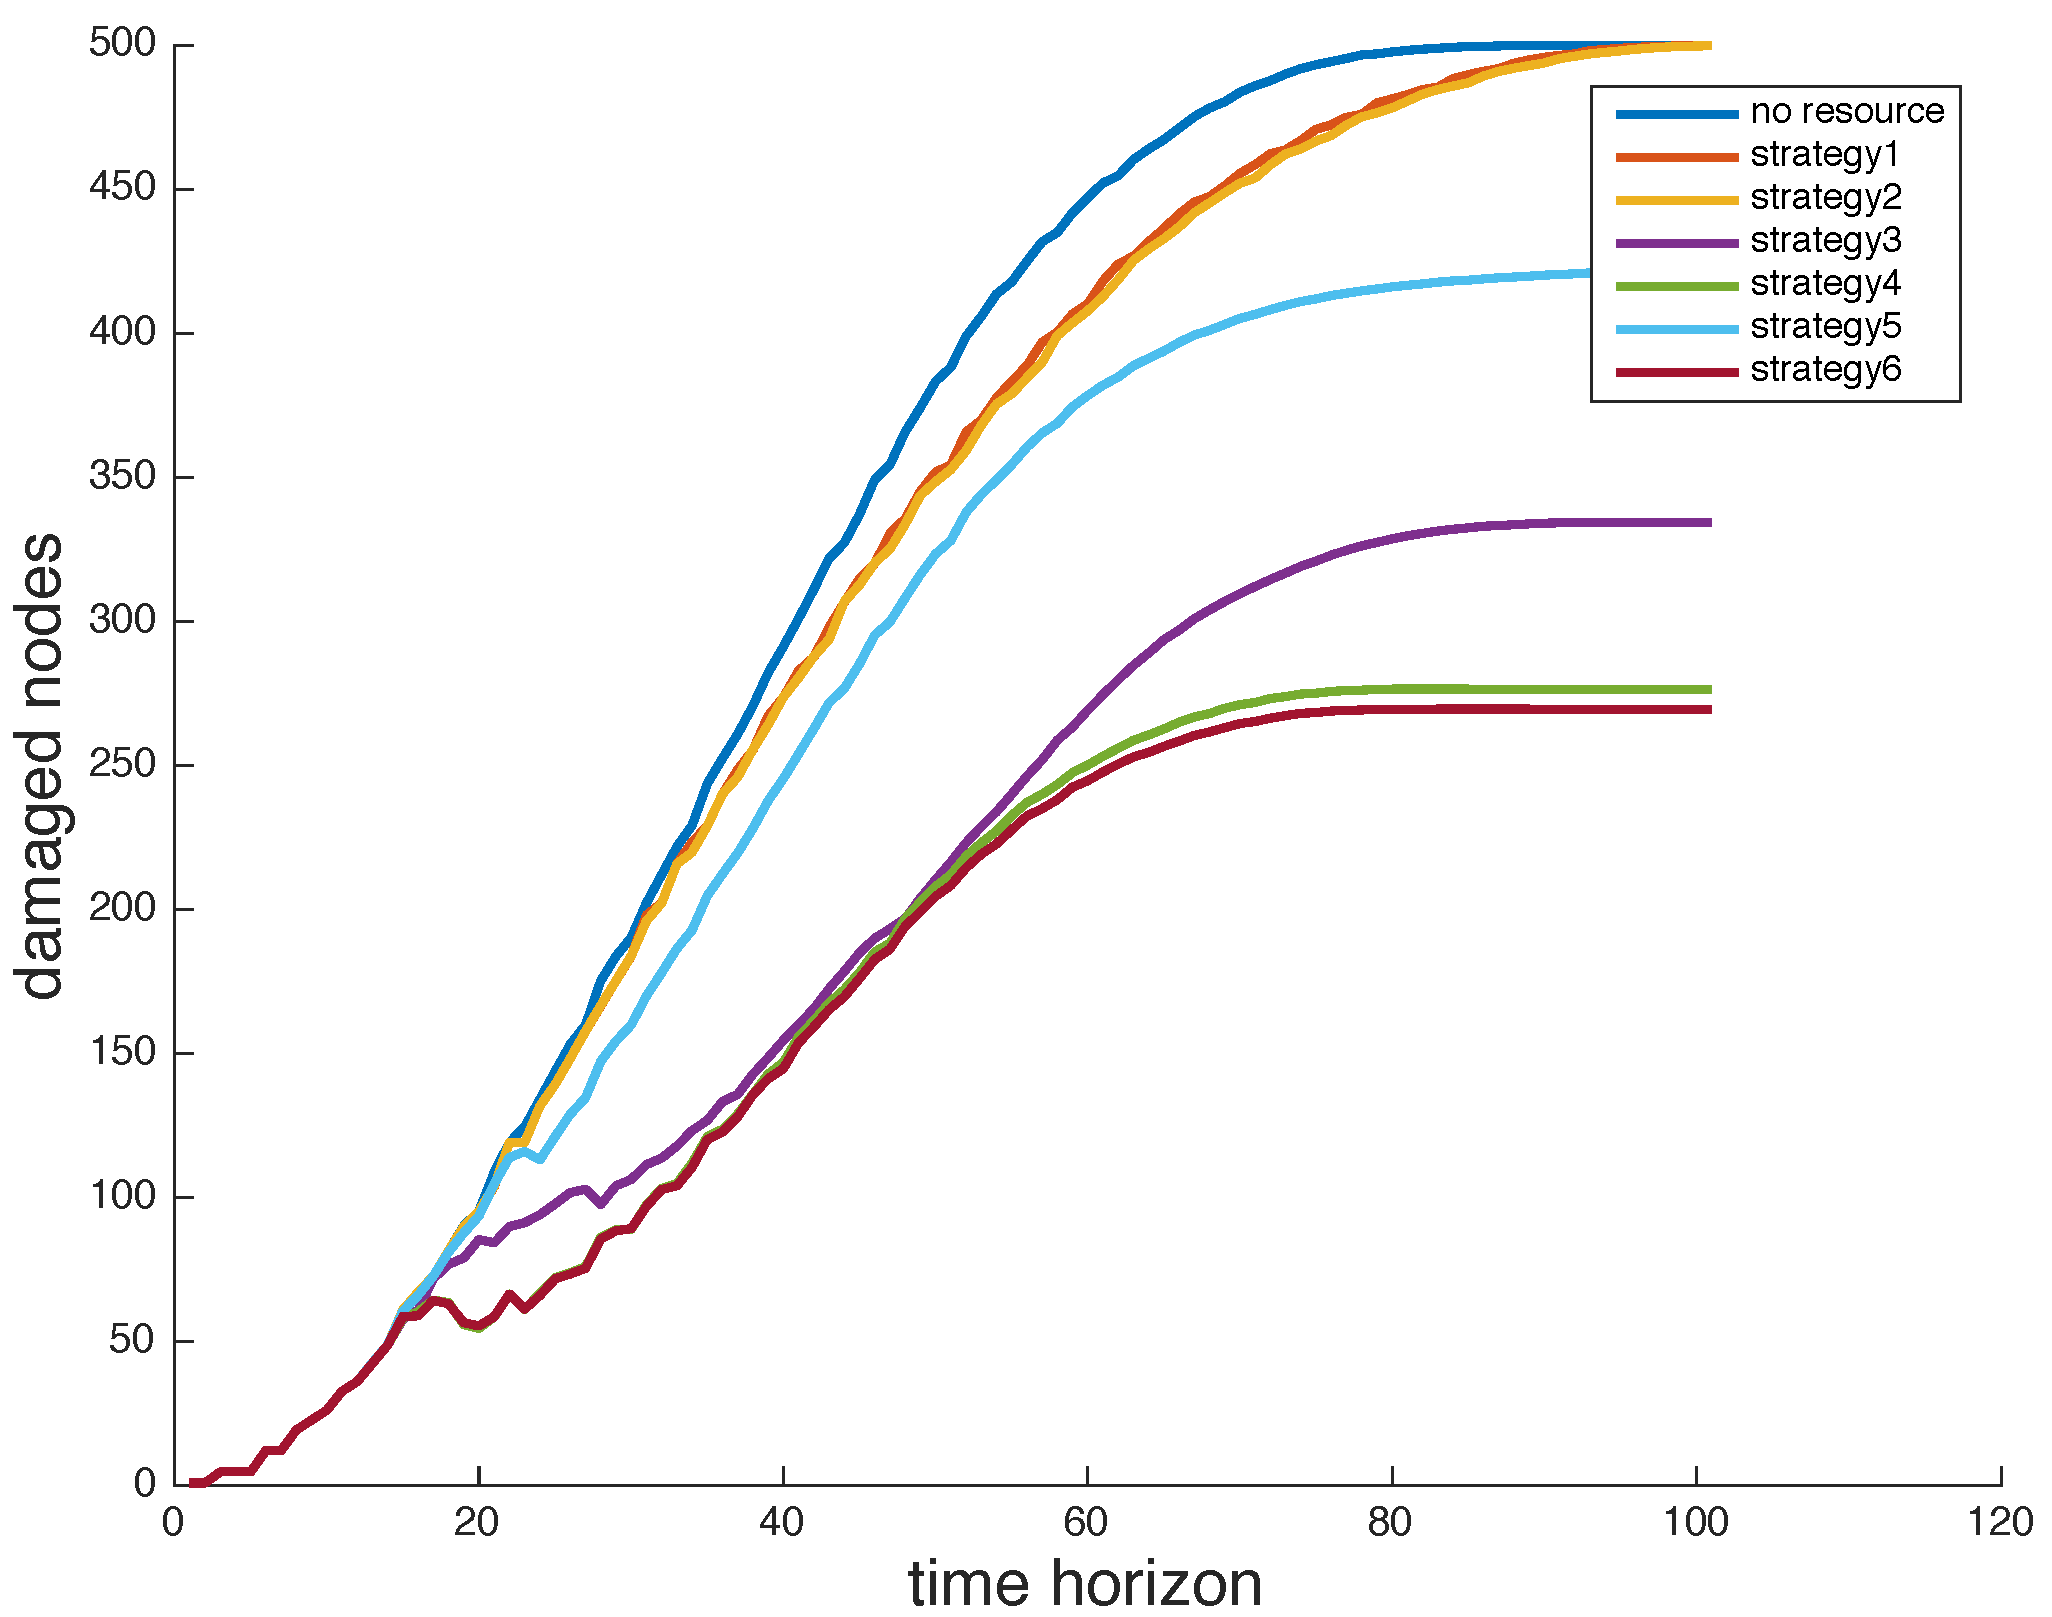
\includegraphics[height=80mm]{../figs/GridNet_original_paper2.pdf}
		\caption{Heuristic strategies on GRID network}
	\end{subfigure}
	~
	\begin{subfigure}[t]{0.8\textwidth}
		\centering
		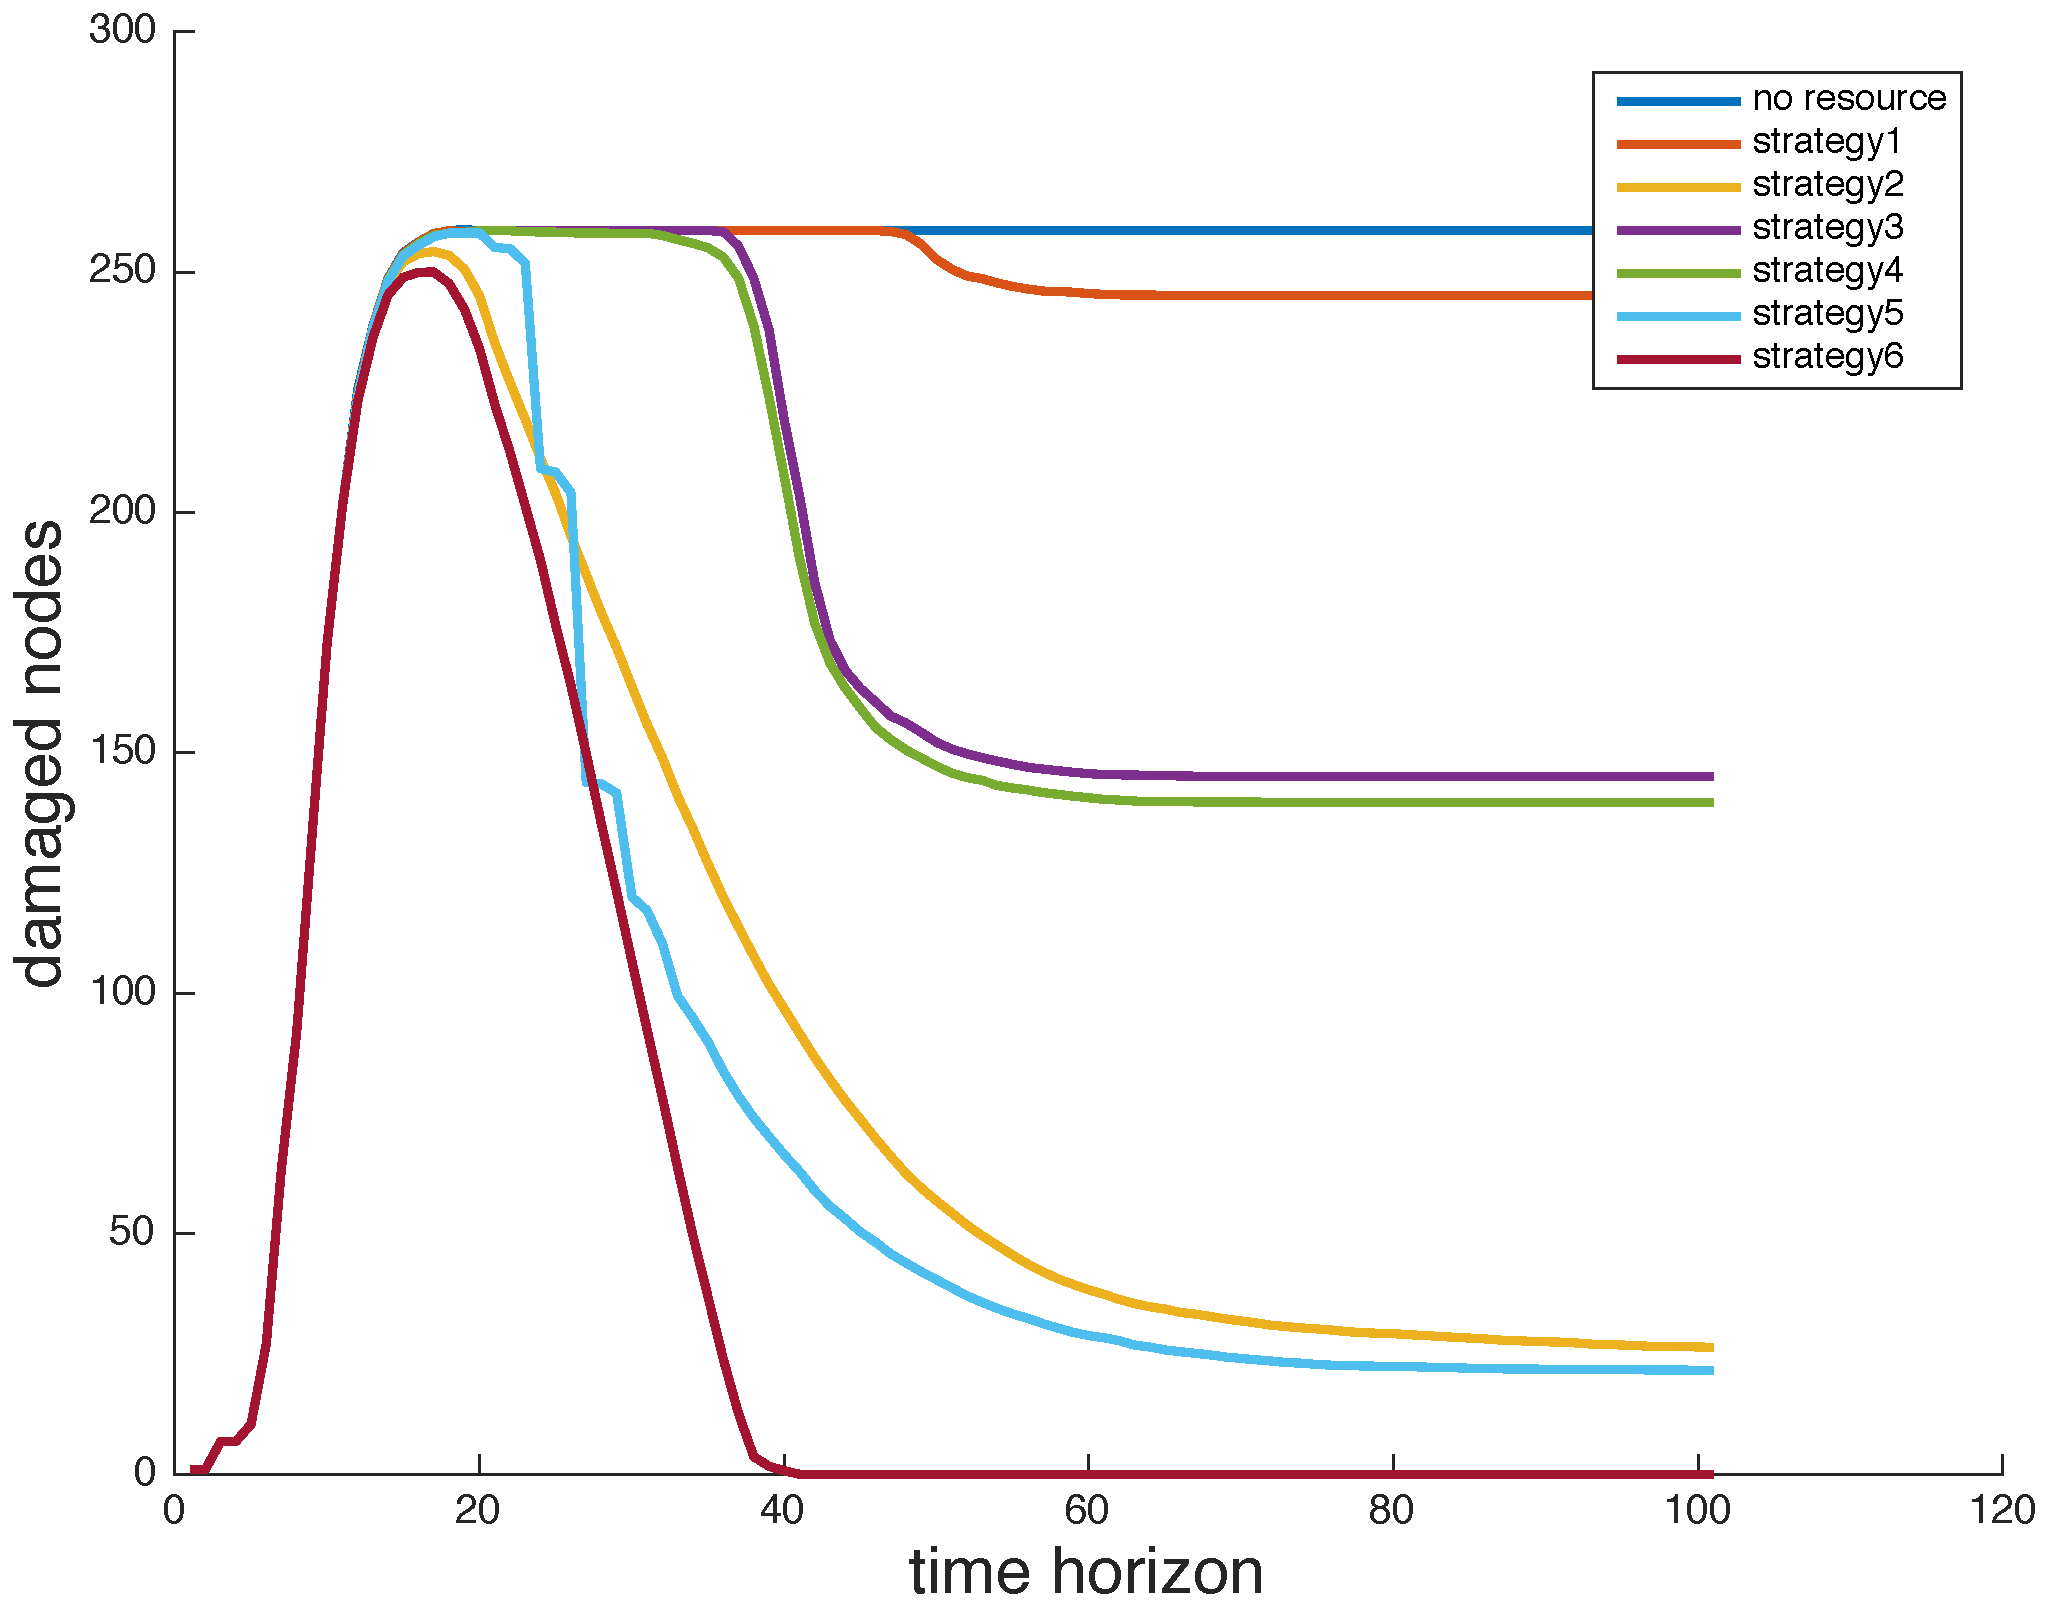
\includegraphics[height=80mm]{../figs/SFNet_original_paper2.pdf}
		\caption{Heuristic strategies on ScaleFree network}
	\end{subfigure}
	\caption{Average number of damaged nodes in (a) grid network and (b) scale-free network, with different heuristic strategis. Total external resources is 1000 and $t_D=8$. The initial damaged node is chosen randomly and these curves is average of 50 experiments.}
	\label{fig:reproduceresult}
\end{figure}
%
One can see that our result (FIG. \ref{fig:reproduceresult}) is almost the same with that in original paper\cite{buzna2007efficient}. During the process of reproducing these results, we have several observations on this disaster spreading model. The most important one is that the spreading process is highly dependent on the choice of initial breaking point. For example in a grid network, a starting node at the center of network will lead to a much more severely damaged final state compared to a starting node at the corner. Due to this reason, we would argue that the averaging among random starting node is meaningless, although we still use this this kind of methodology for comparison in this report. We would suggest to discuss the effect of initial damaged node's location on the spreading of disasters in future research. We also notice that in both grid and scale-free networks, S6 has the best performance. This is easy to understand because to conduct S6, we require more information than in other strategies and distribute resources with consideration of each node's status. From this observation, we can infer that more detailed information of the network topology and nodes' status will admit a better strategy. In another word, we can find an optimal strategy is we have full information on the network topology and nodes' properties. And this will be main result of the this report.

\subsection{The Optimal Strategy}
We have introduced our optimization method in Sec. \ref{sec:adjointmethod}, and we will show our results in this section. Details about setups of our model will be shown in Appendix \ref{sec:appendix1} and \ref{sec:appendix2}. 

\subsubsection{Minimize The Number of Damaged Nodes}
As anticipated in section \ref{sec:methods}, we originally want to minimize the number of damaged nodes after a certain time window $T$. This is also the base idea used in \cite{buzna2007efficient}. This choice is very natural because we want to control the number of damaged nodes, i.e. in our model the number of nodes $x^{(i)}_T>\theta_i$ after spreading of a disaster. Intuitively an objective function for this purpose is the $0-1$ loss function:

\begin{equation}
	\label{eq:0_1_loss}
	\begin{aligned}
		J &= \sum_i h(x_i) \\
		\text{where } h(\cdot) &= 
		\begin{cases}
			1 & \text{if } x_i \ge \theta_i \\
			0 & \text{otherwise}
		\end{cases}
	\end{aligned}
\end{equation}

However, discontinuity of this function will be a problem when we take variance of the Lagrangian. To solve this we introduce another objective function to approximate the $0-1$ loss function. 

\begin{equation}
	\label{eq:sigmoid2}
	\begin{aligned}
		J &= \sum_i \Phi_i(x_i) \\
		\text{where } \Phi_i(y) &= \frac{1-\exp(-\alpha y)}{1+\exp(-\alpha (y-\theta_i))}
	\end{aligned}
\end{equation}

Sigmoid functions with respect to different values of $\alpha$ are shown in Fig. \ref{fig:sigmoid_alpha}. We find that a sigmoid function with $\alpha$ set to $20$ can approximate the $0-1$ loss function very well. So we set $\alpha=20$ in our model. By this function, we expect that optimized strategy will give a lower number of damage nodes than any other strategies. Fig. \ref{fig:opt_on_grid}(a) shows the evolution of number of damaged nodes with respect to different strategies proposed in \cite{buzna2007efficient} and the optimized solution on a grid network. The same result on a scale-free network is shown in Fig. \ref{fig:opt_on_sf}(a).  It is clear that the optimized solution is better than any other heuristic strategies. It is worth to mention that, due to nature of the chosen objective function, a random starting resources distribution strategy will not be a good choice. This is because almost all nodes are above $\theta_i$ and locate and the right flat part of sigmoid function, so the gradient is almost zero here.  However we have a natural choice of starting model, say \textbf{S6} in a grid network. Although this choice makes optimization numerically possible, we are still faced with the problem of very small gradient and many local minimums. There is no guarantee that this optimal solution in our plot is a global minimum and we believe that this solution can still be improved by using more suitable numerical  techniques. 

\begin{figure}
	\centering
	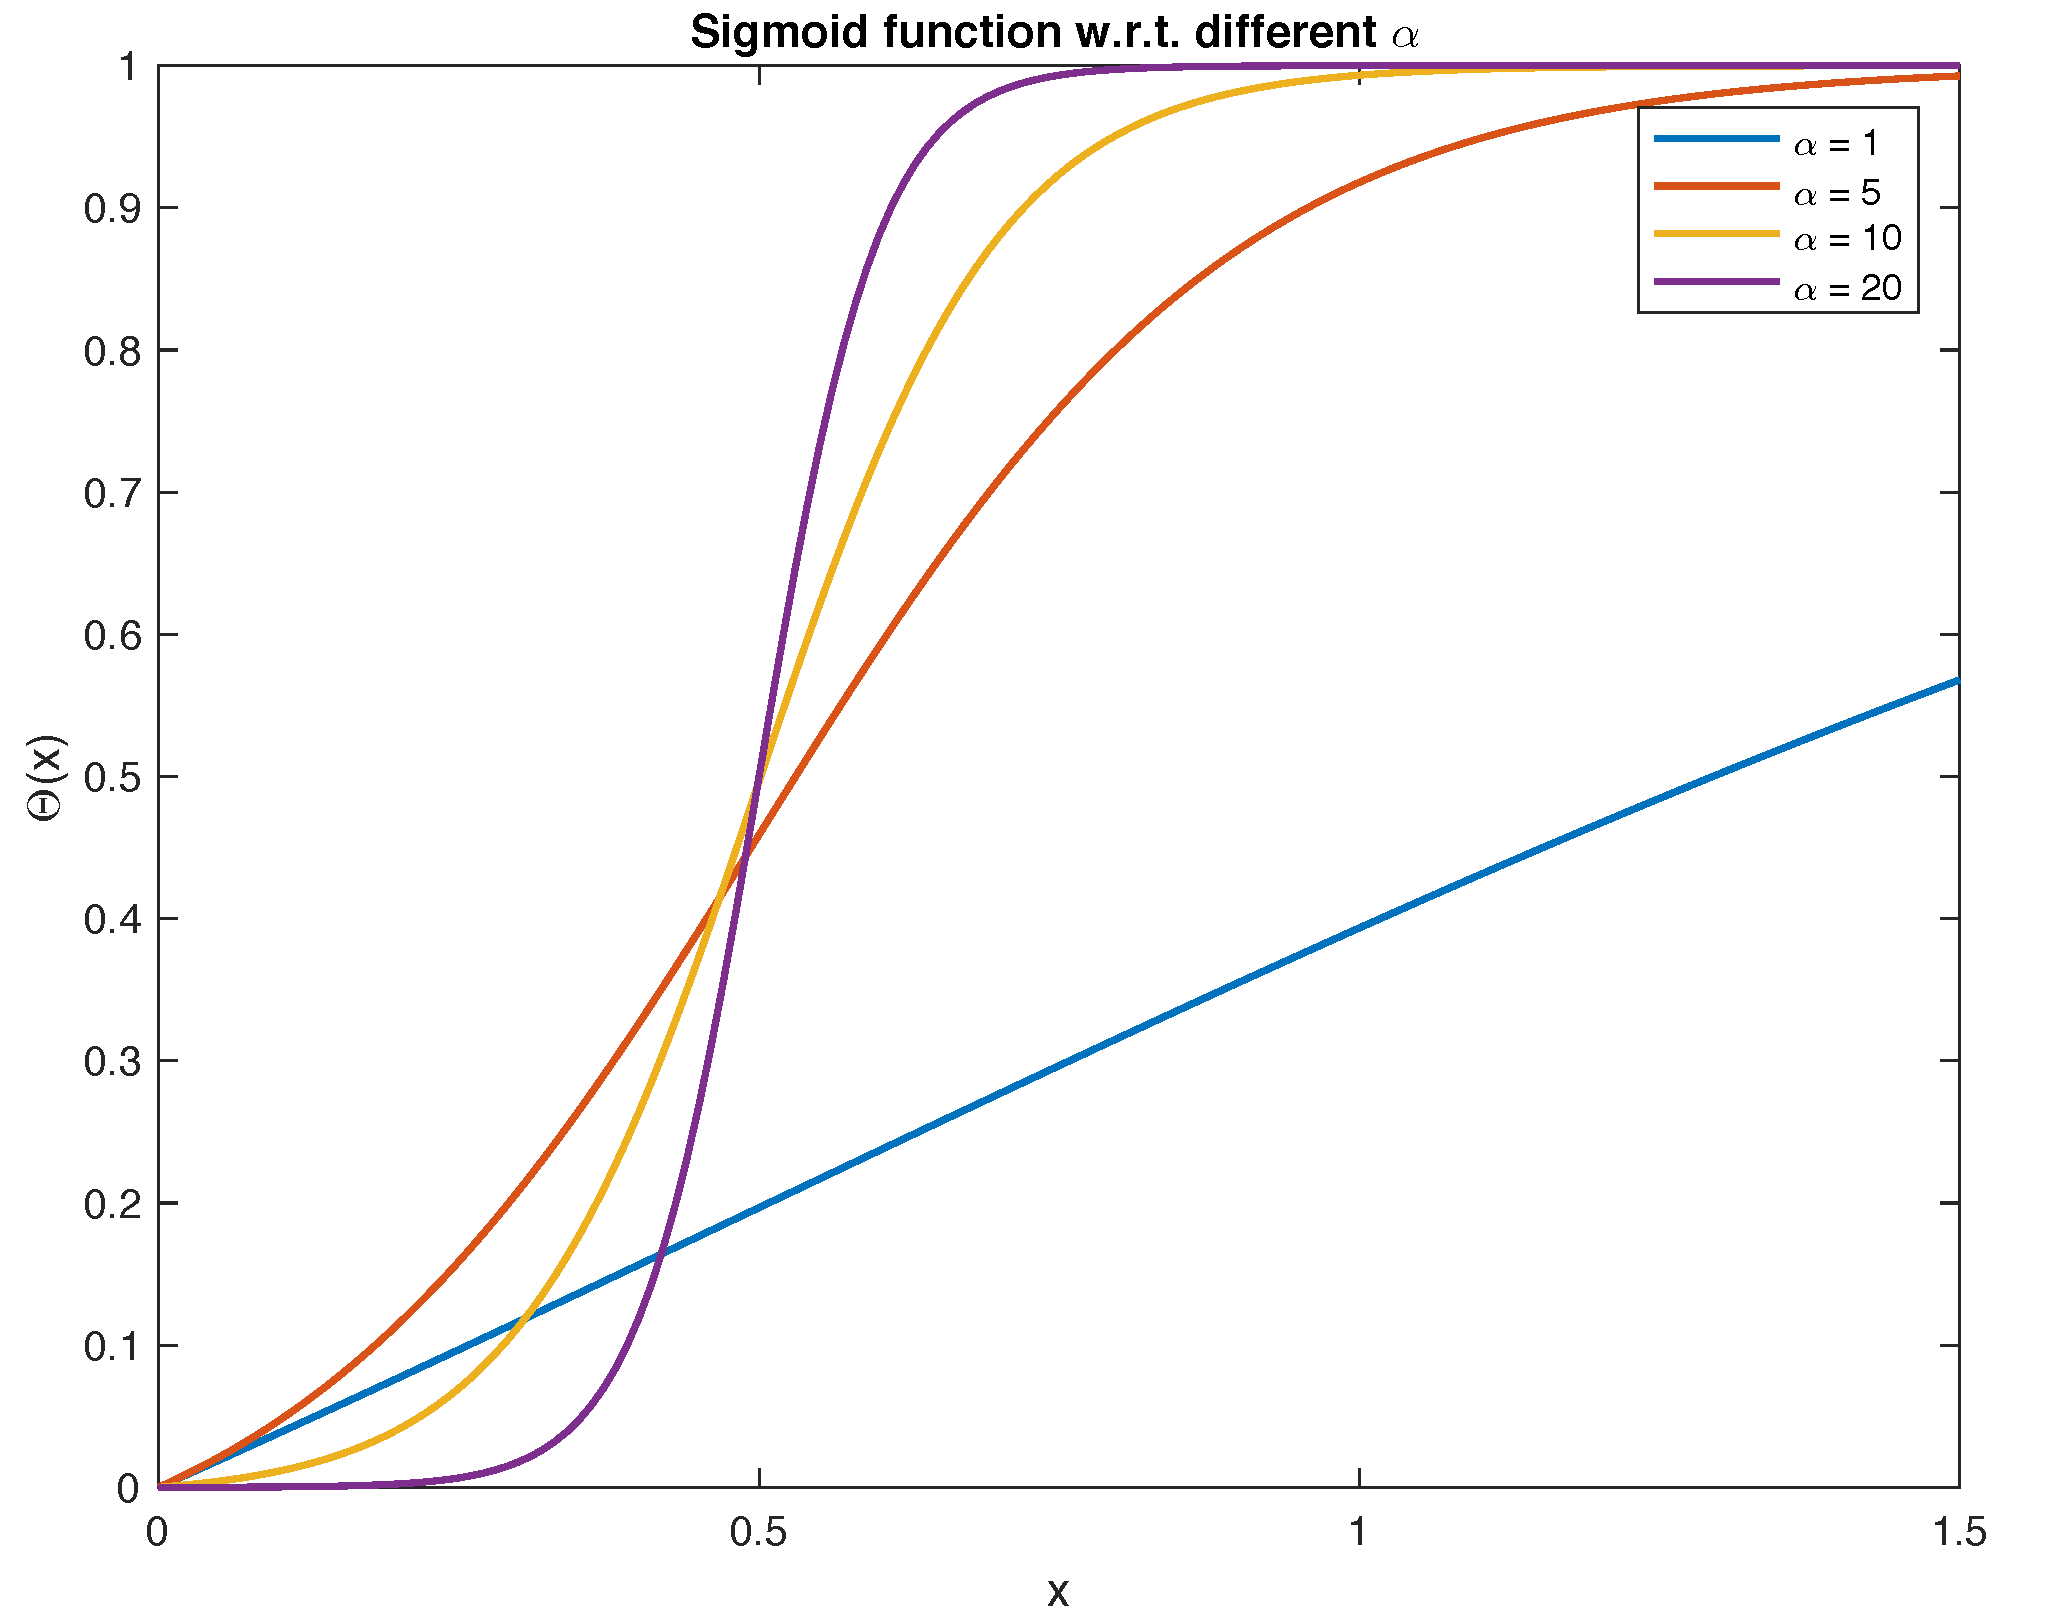
\includegraphics[height=60mm]{../figs/sigmoid_small.pdf}
	\caption{Shape of sigmoid function w.r.t. different $\alpha$. $\theta$ is set to $0.5$. When $\alpha=20$, this function gives a very good approximation of the $0-1$ step function.}
	\label{fig:sigmoid_alpha}
\end{figure}

\begin{figure}
	\centering
	\begin{subfigure}[t]{0.8\textwidth}
		\centering
		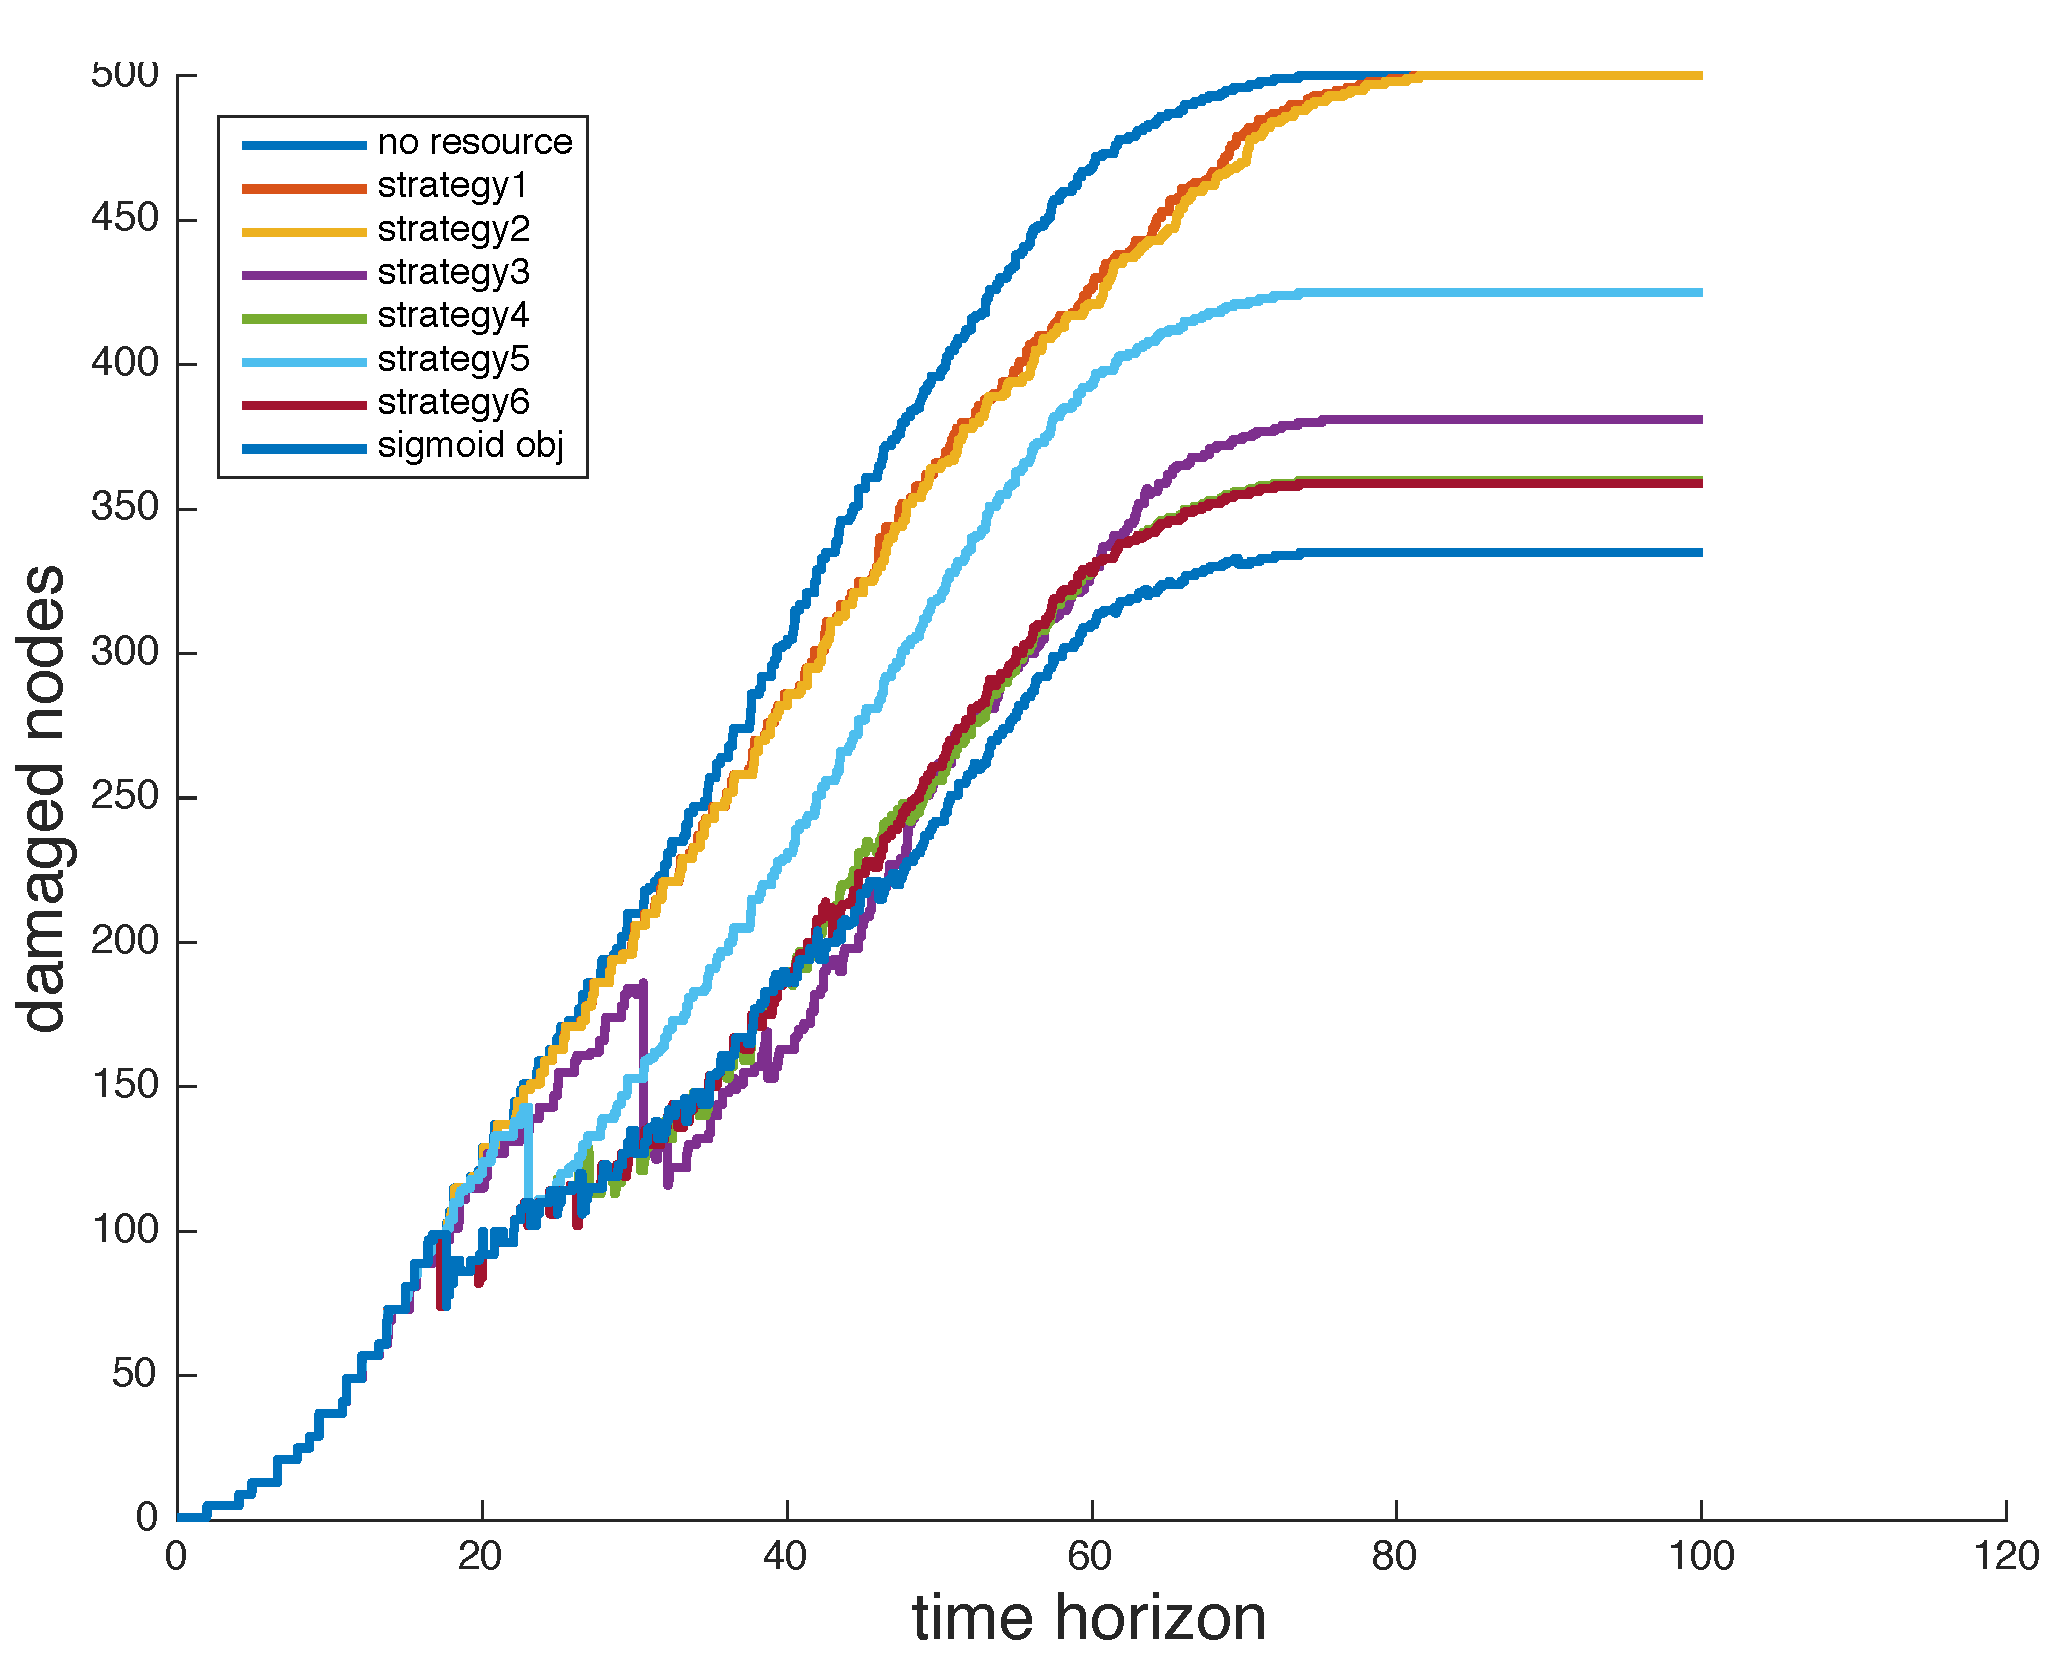
\includegraphics[height=80mm]{../figs/no_linear_approximation/Grid_damaged_small.pdf}
		\caption{Damaged nodes on grid network}
	\end{subfigure}
	~
	\begin{subfigure}[t]{0.8\textwidth}
		\centering
		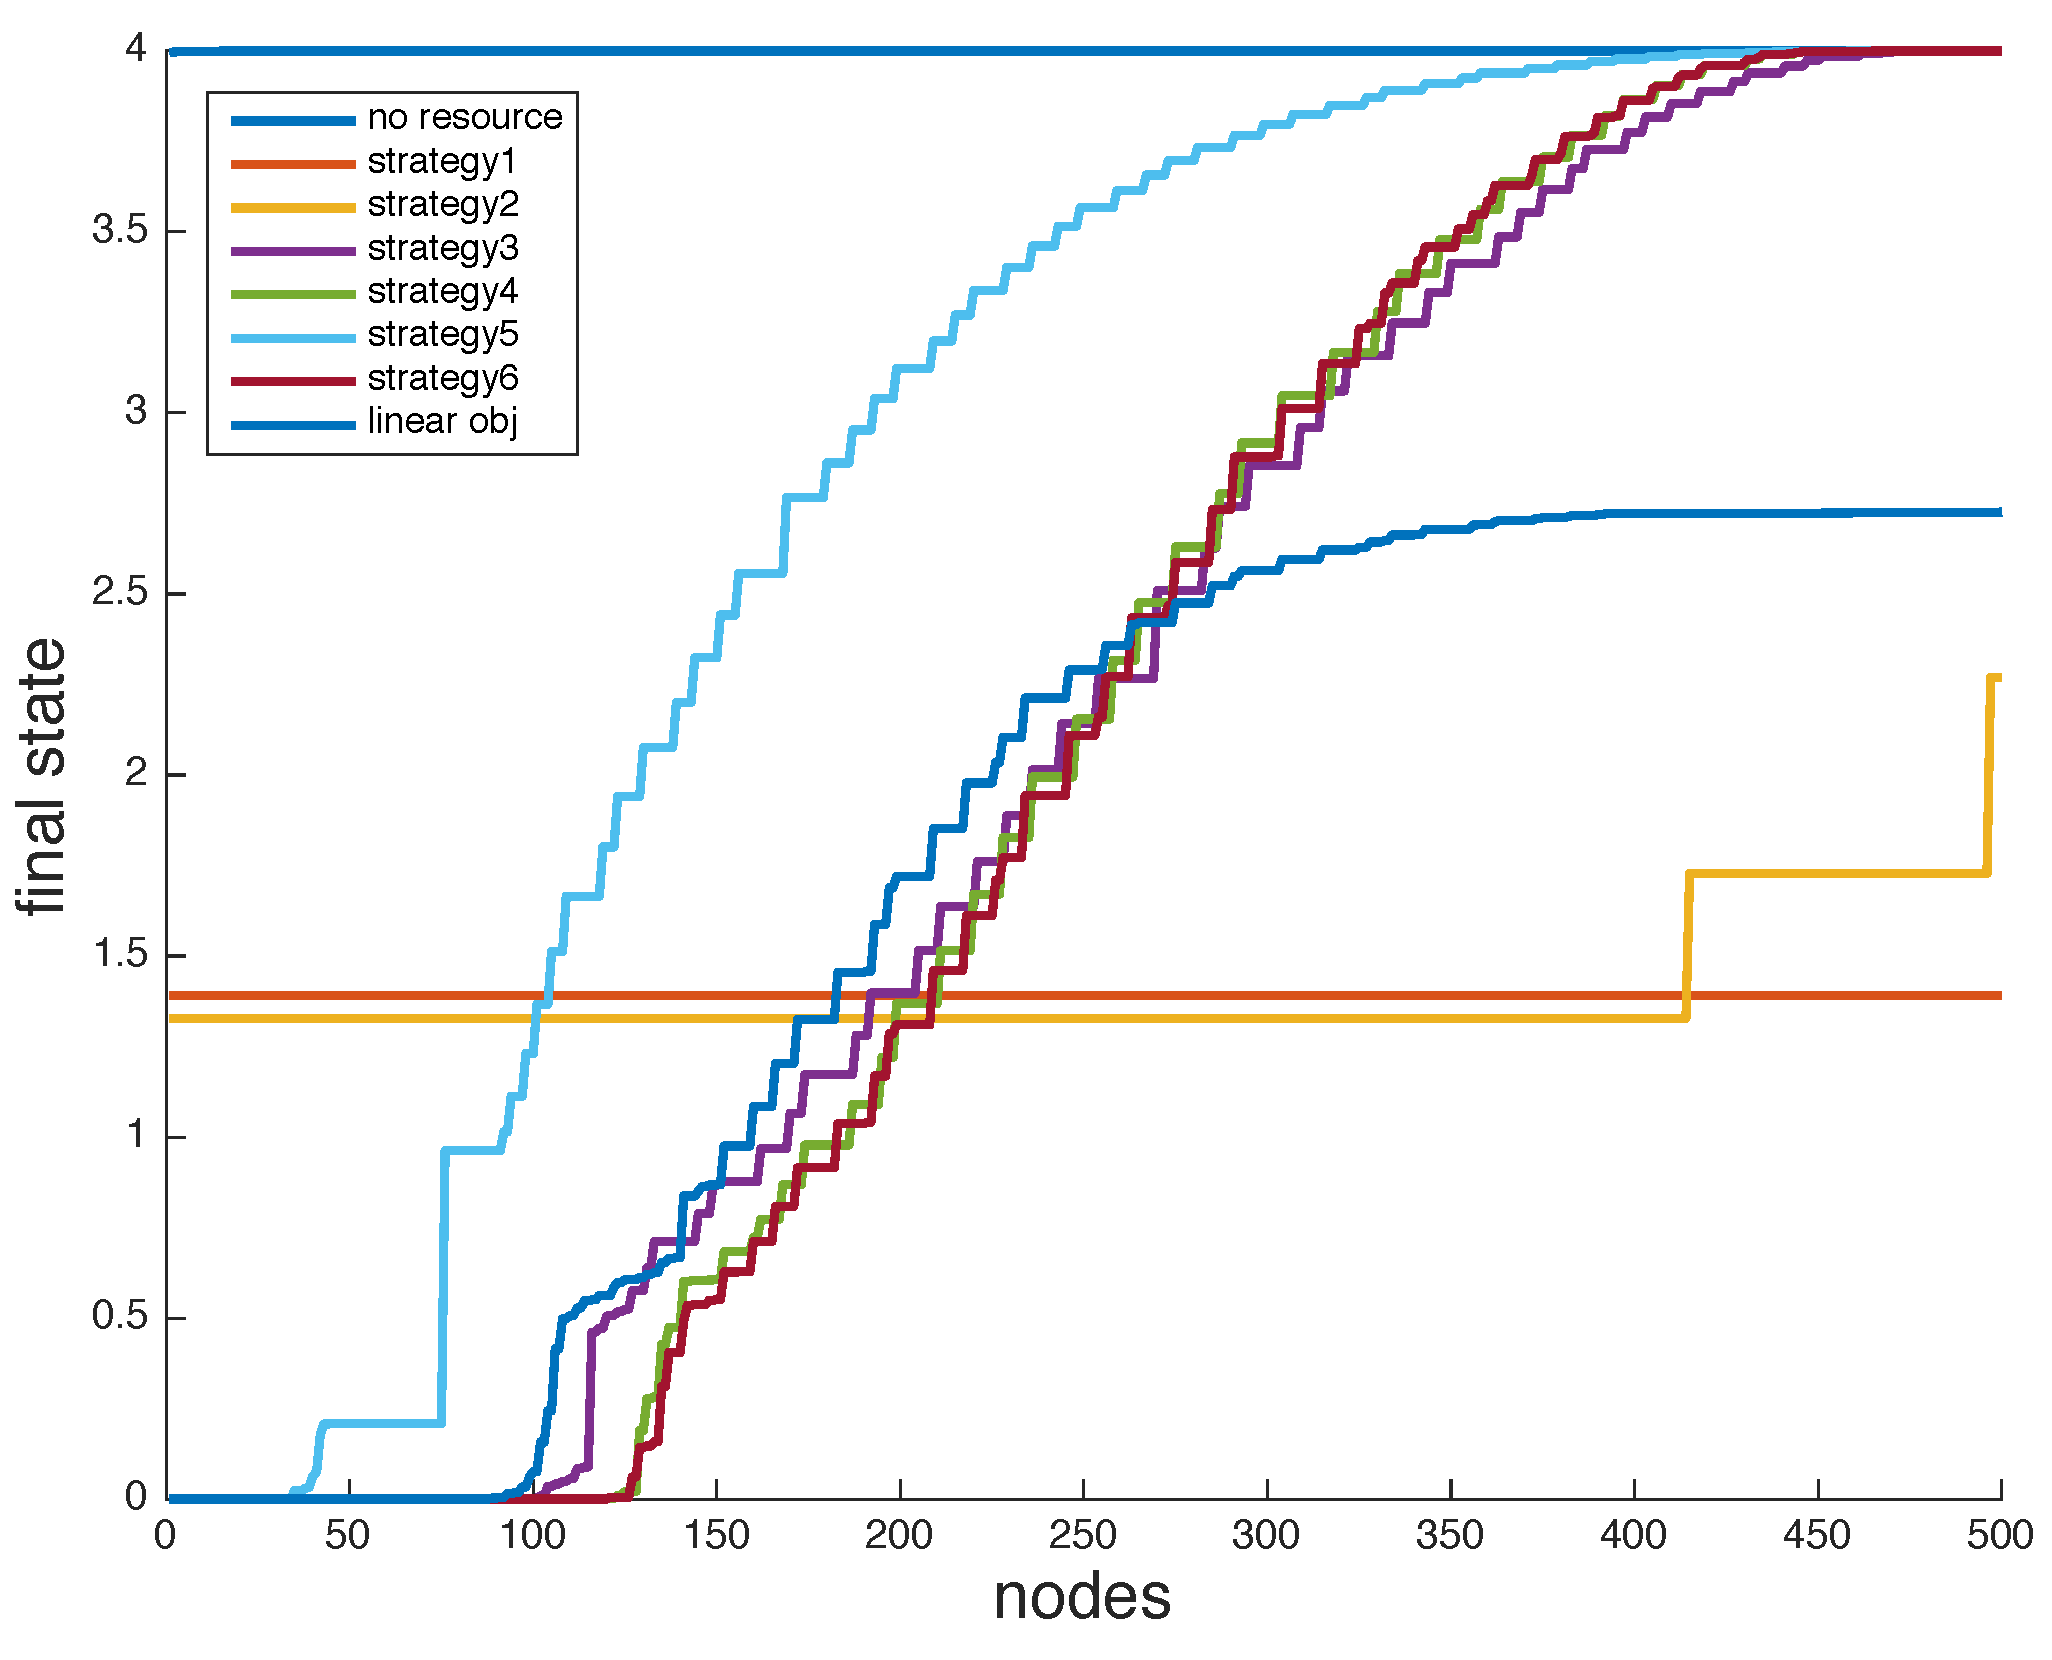
\includegraphics[height=80mm]{../figs/no_linear_approximation/Grid_finalState_small.pdf}
		\caption{Final states on grid network}
	\end{subfigure}
	\caption{(a) Number of damaged nodes and (b) final states on grid network. Total external resources is 1000 and $t_D=8$. The initial damaged node is chosen randomly. The maximal iterations of gradient descent is 100.}
	\label{fig:opt_on_grid}
\end{figure}

\begin{figure}
	\centering
	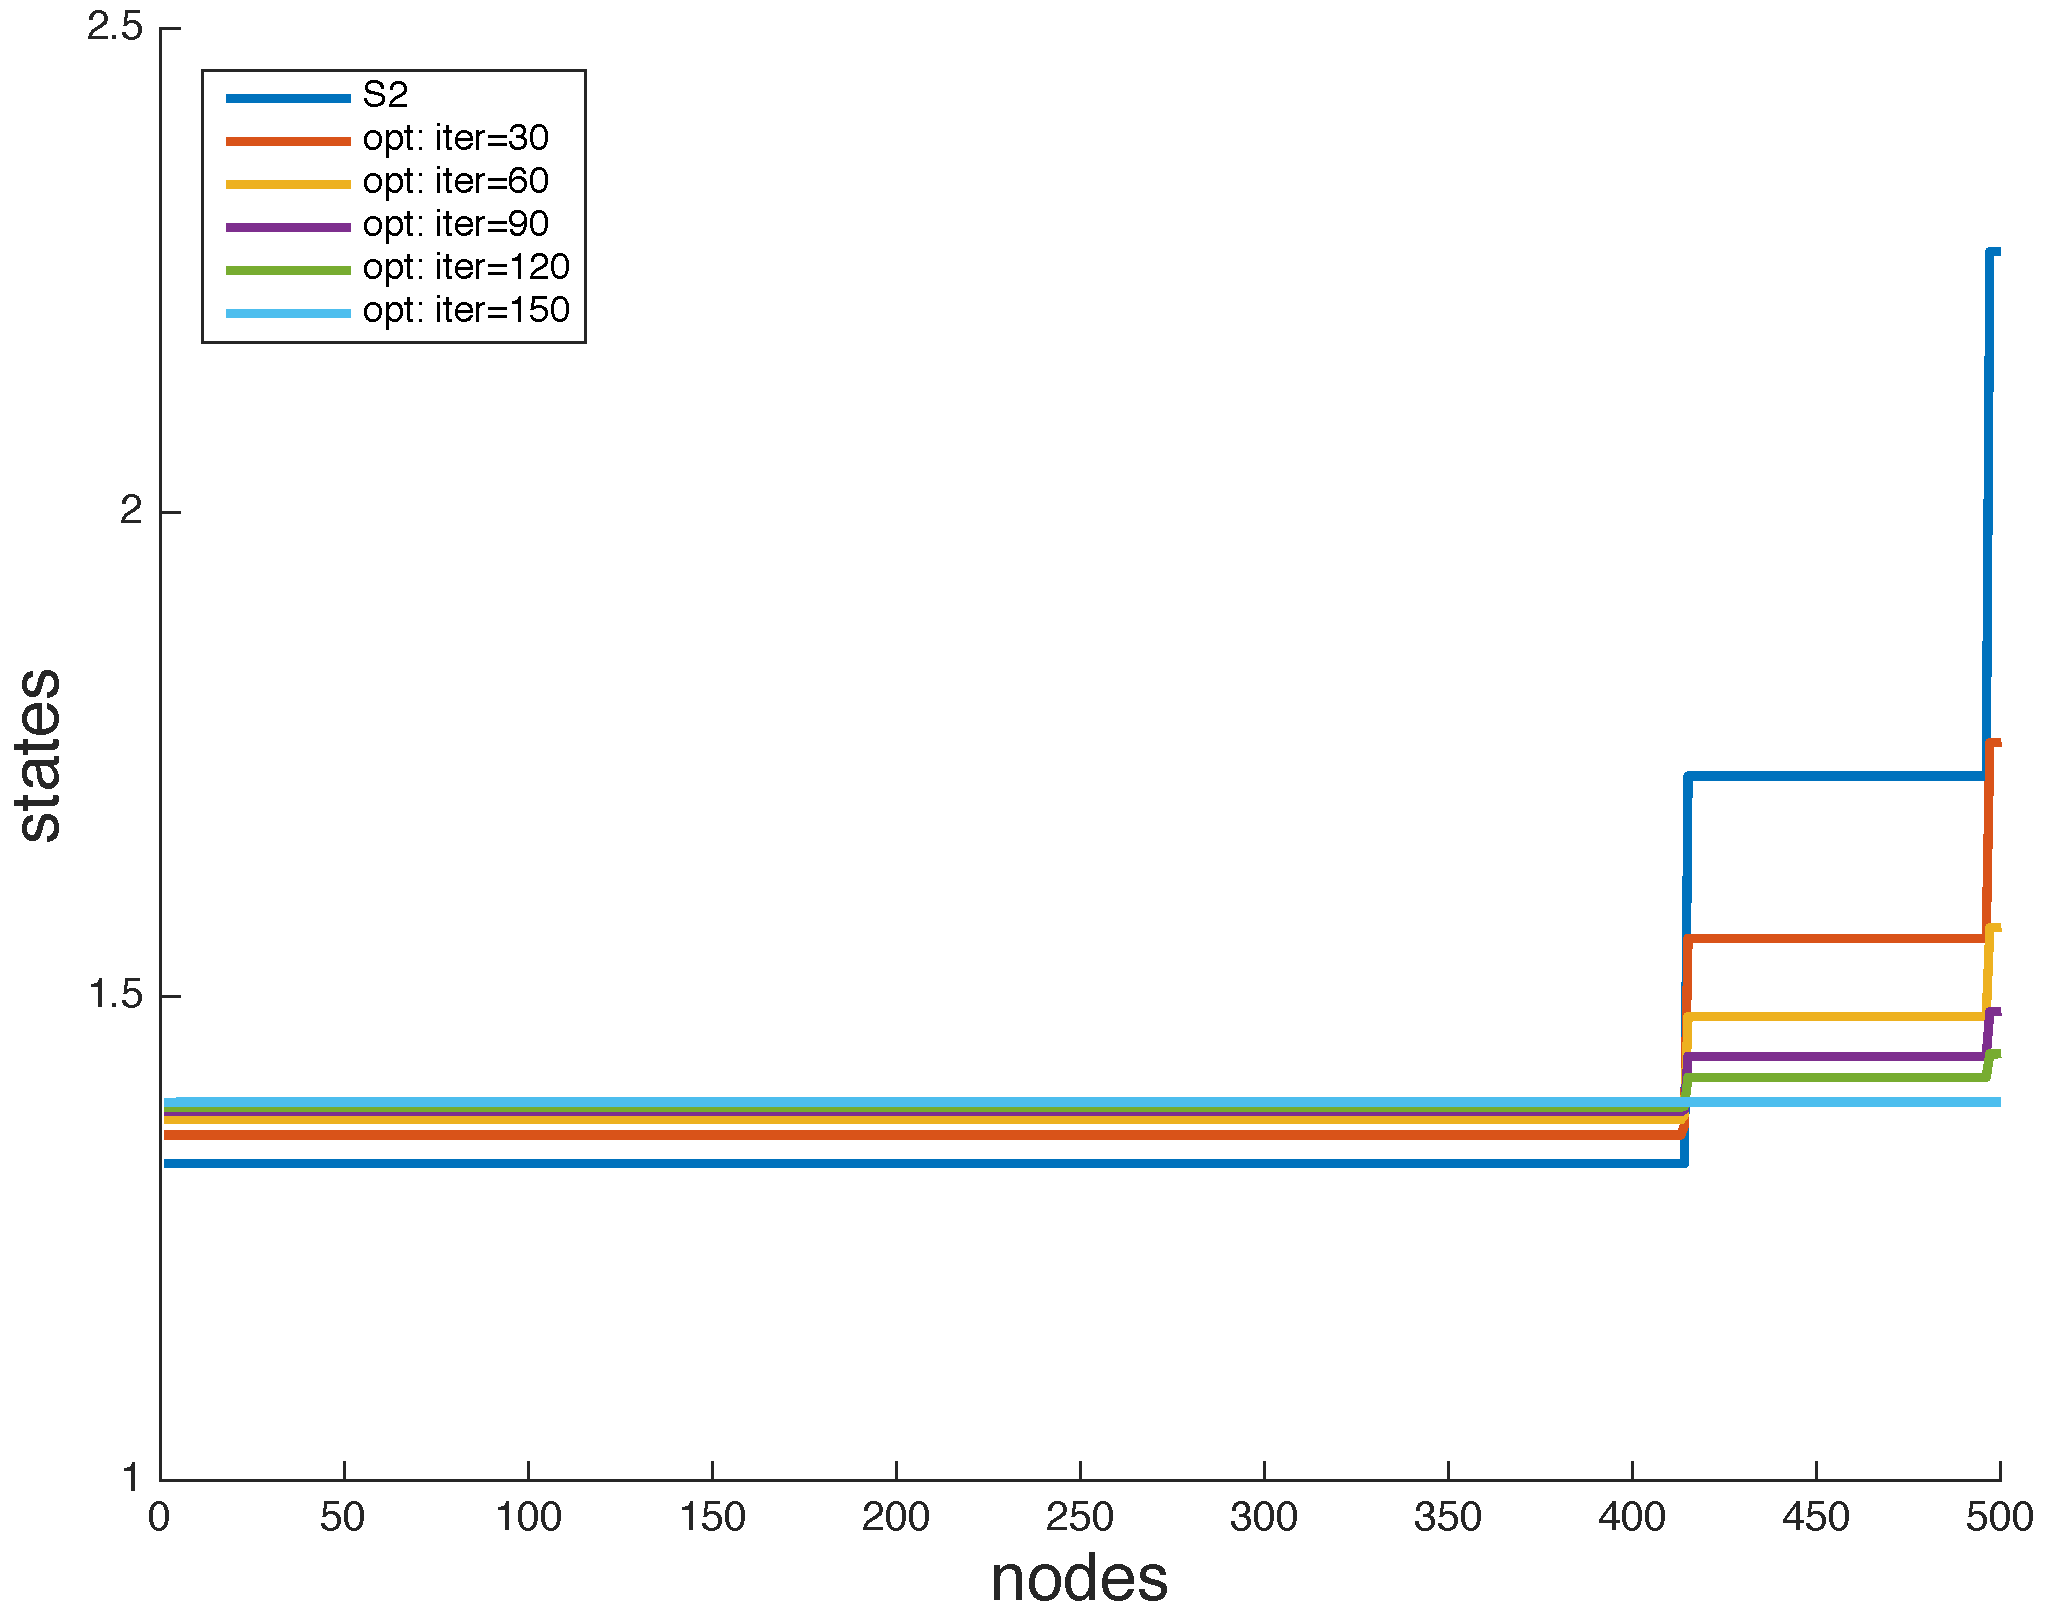
\includegraphics[height=60mm]{../figs/grid_optimal_from_S2/Grid_OptimalStates_small.pdf}
	\caption{States of optimal strategy at different time, optimized from \textbf{S2}. We can find that the optimal solution converges to \textbf{S1}}
	\label{fig:opt_from_S2}
\end{figure}

\begin{figure}
	\centering
	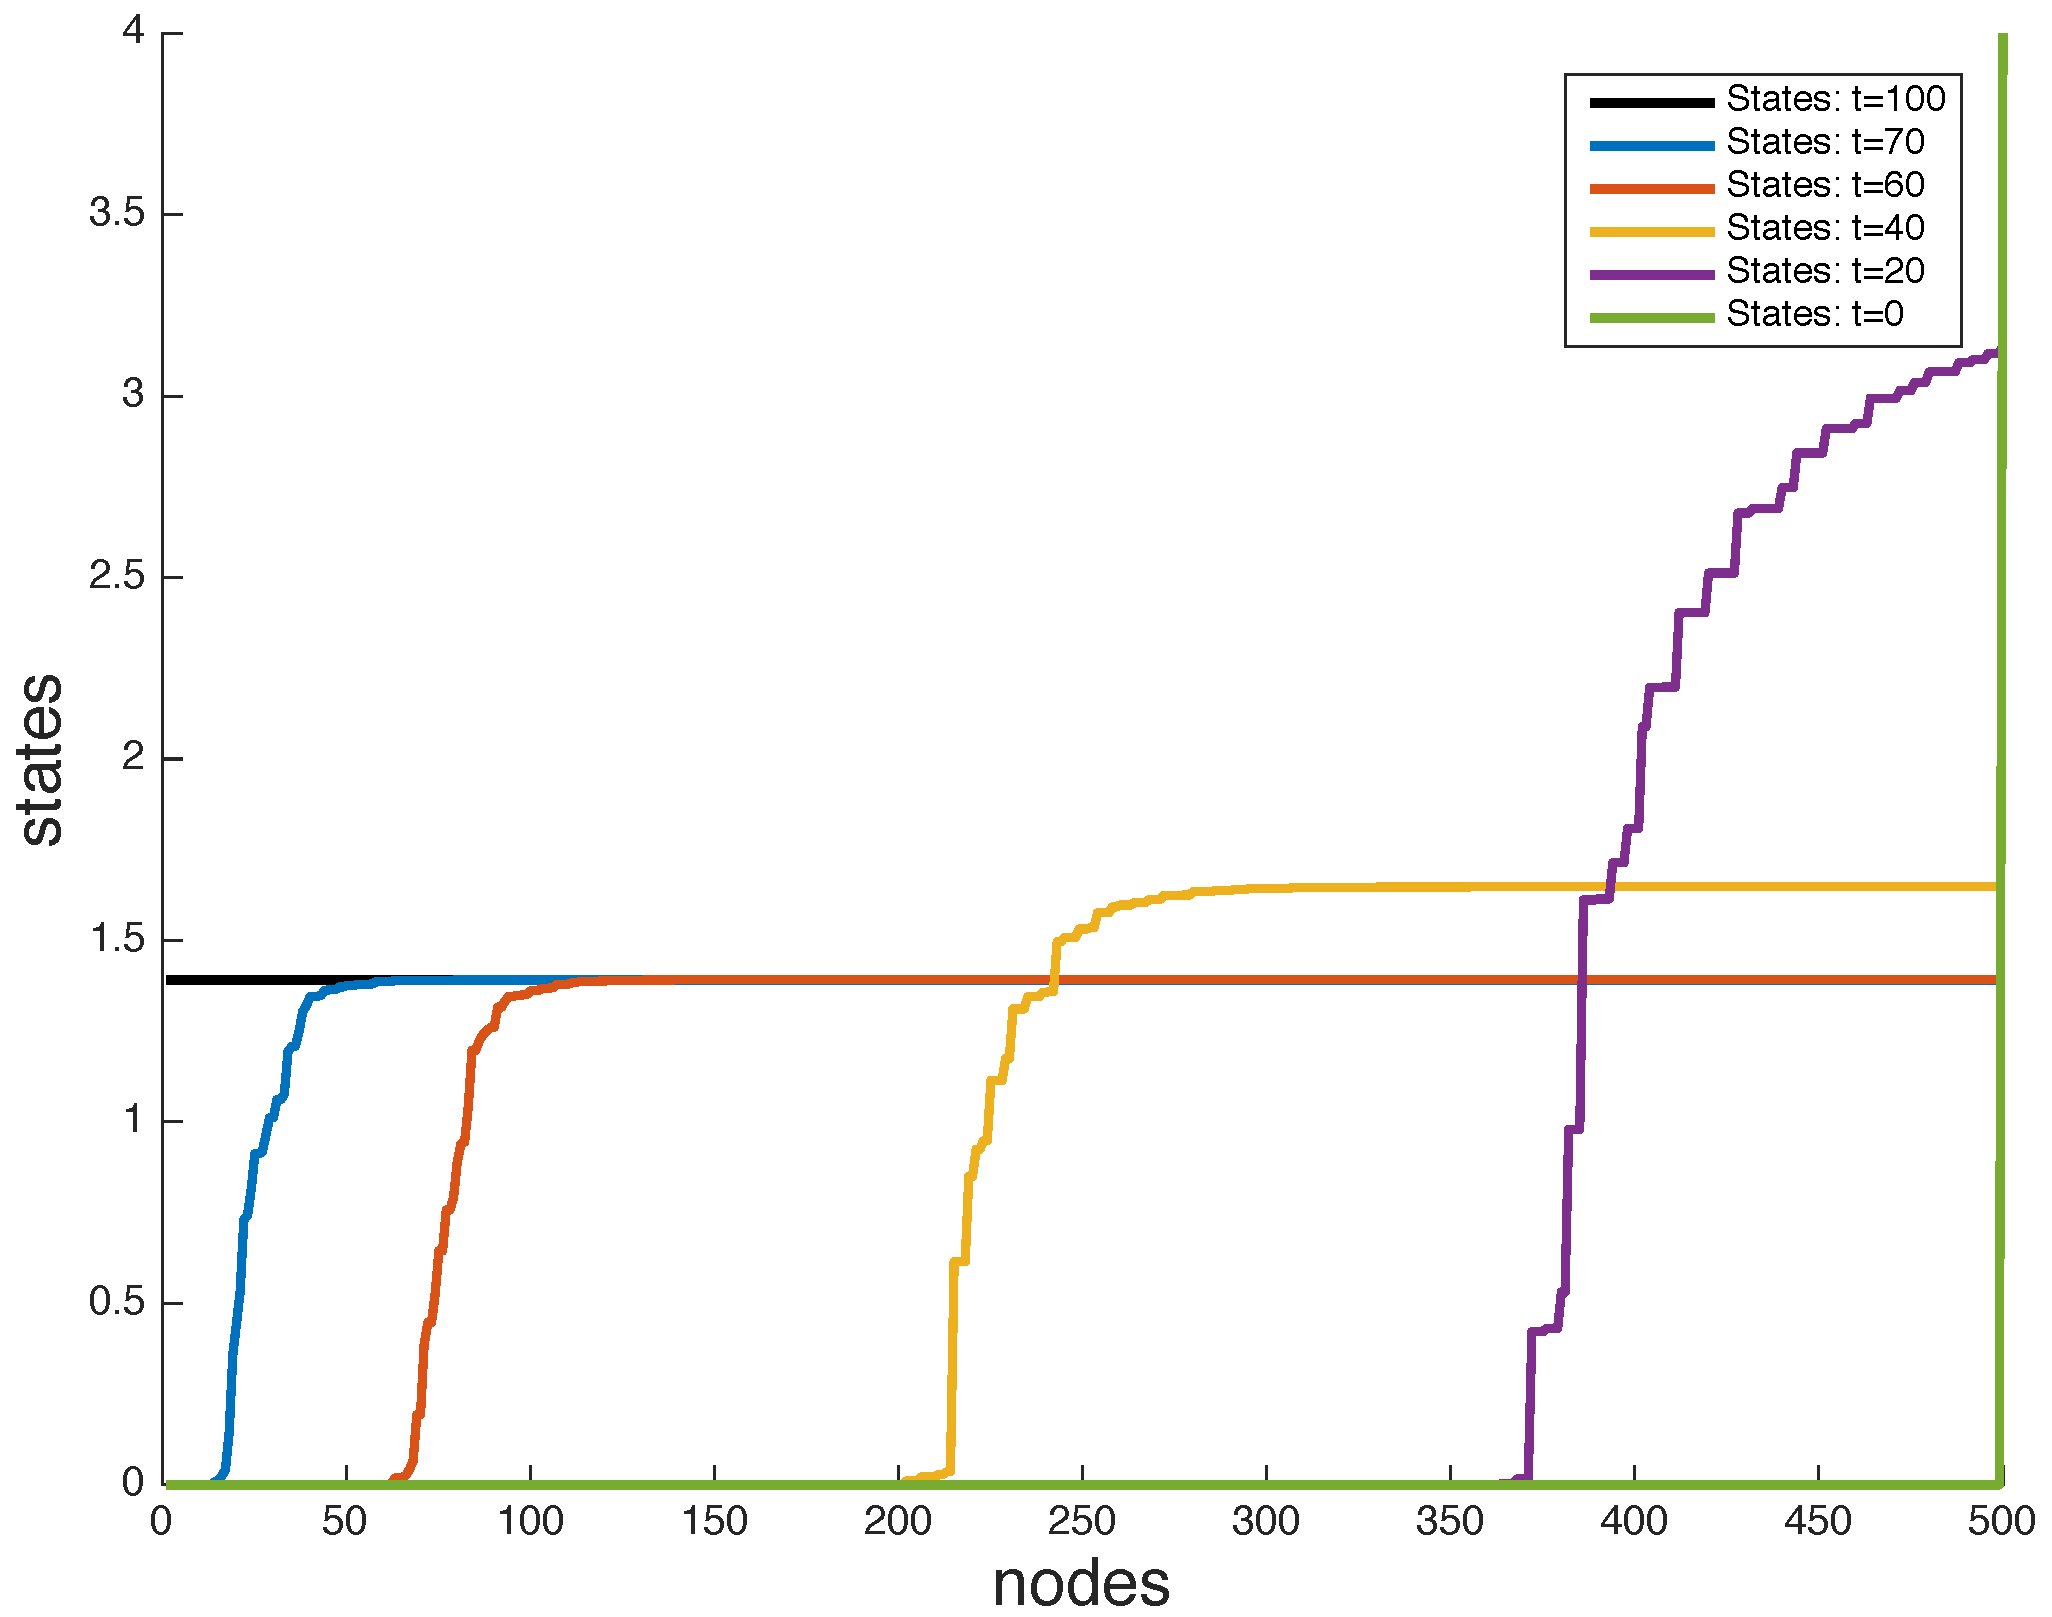
\includegraphics[height=60mm]{../figs/grid_optimal_from_S2/Grid_S1_States_small.pdf}
	\caption{Nodes' states of \textbf{S1} at different time steps. We find the whole system comes to a stable state.}
	\label{fig:zhichao}
\end{figure}

\subsubsection{Optimize Final States}
In Fig. \ref{fig:opt_on_grid}(b) and \ref{fig:opt_on_sf}(b) we plot the final state of each nodes in an ascending way. One can see that although the number of damaged nodes is controlled by those strategies such as \textbf{S6}, some nodes persist very high status value. In real world, it would imply that those components of the network is badly damaged for a very long time. One can argue that this kind of situation is not acceptable and want to avoid those very badly damaged nodes. This is exactly the starting point of our choice of a second objective function as:


\begin{equation}
\label{eq:obj2}
	J = \frac{1}{n} \sum_i x_T^{(i)}
\end{equation}

Eq. (\ref{eq:obj2}) aims at optimizing the average final state of all nodes. It exclude the situation that some nodes are severely damaged. The optimized strategies on grid network and scale-free network are shown in Fig. \ref{fig:opt_on_grid}(b) and Fig. \ref{fig:opt_on_sf}(b) respectively. On scale-free network our optimal gives a better strategy compared to all other ones, while on a grid network one may see that the optimal solution is exactly the one comes from S1. We would interpret this as that $T=100$ is long enough for S1 and S2 to reach a stable state, and in this case S1 is indeed the best one. We can explain this qualitatively. The time window is long enough and the system arrive at the stable state and due to the nature of grid-network,  the local topology of each node is almost the same. So we would speculate that when arriving at a stable state, all nodes must have similar status. However if performing some simple analysis on the definition of recover rate, one would find that distribute resources equally would be the best solution under those assumptions above. We also proved this numerically. In Fig. \ref{fig:opt_from_S2}, we show that if we start our optimization from S2, we arrive at exactly the result of S1. Also, to show that results from S1 is a stable solution, we show the evolution of nodes' status at several time steps in Fig. \ref{fig:zhichao}.  One can also see that the optimal solution in this case might also be unsatisfactory. This objective function will more likely lead to averaging state of all nodes. When total resource is very limited, this strategy will result that almost all nodes are damaged, although not in a very bad way. 

So we can conclude from our optimization that the more we know about the network system, the better we can distribute the resources. In general, the best strategy depends on the objective we want to achieve, especially when resource is limited. Although objective functions may differ, our observation is that decision makers need to identify those highly risky nodes and distribute suitable amount of resources in advance to prevent the spreading of disasters, rather than after a certain node is damaged already.  


\begin{figure}	
	\centering
	\begin{subfigure}[t]{0.8\textwidth}
		\centering
		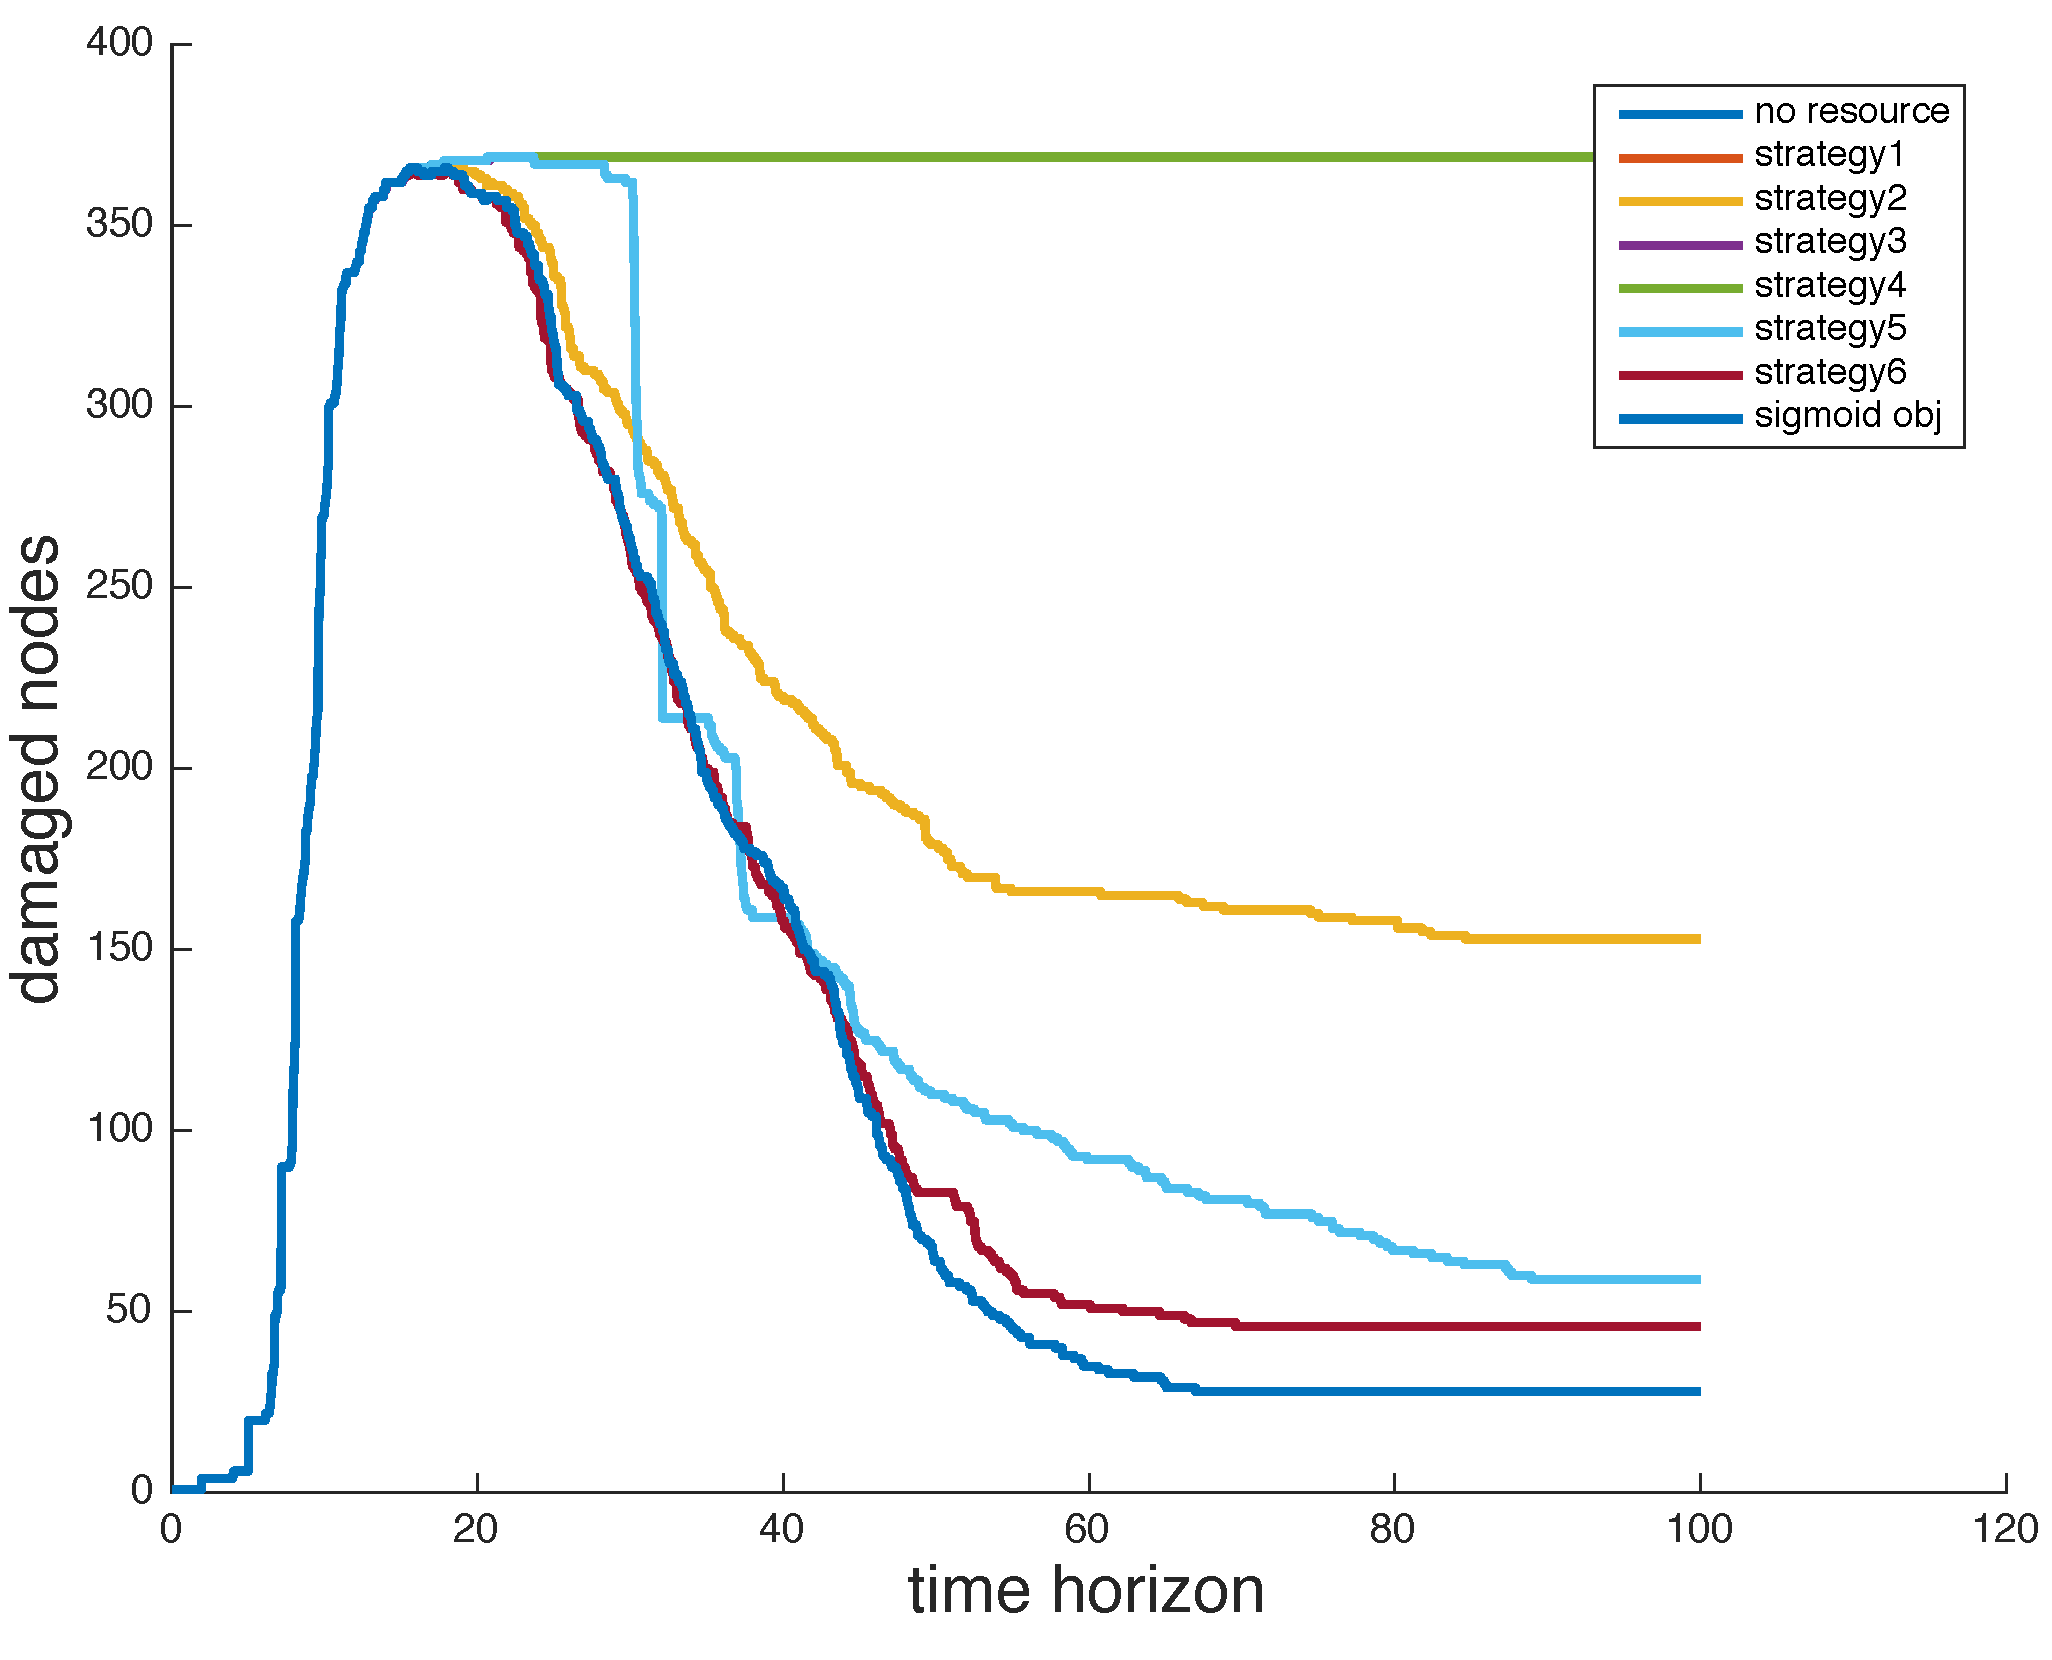
\includegraphics[height=80mm]{../figs/no_linear_approximation/SF_damaged_small.pdf}
		\caption{Damaged nodes on scale-free network}
	\end{subfigure}
	~
	\begin{subfigure}[t]{0.8\textwidth}
		\centering
		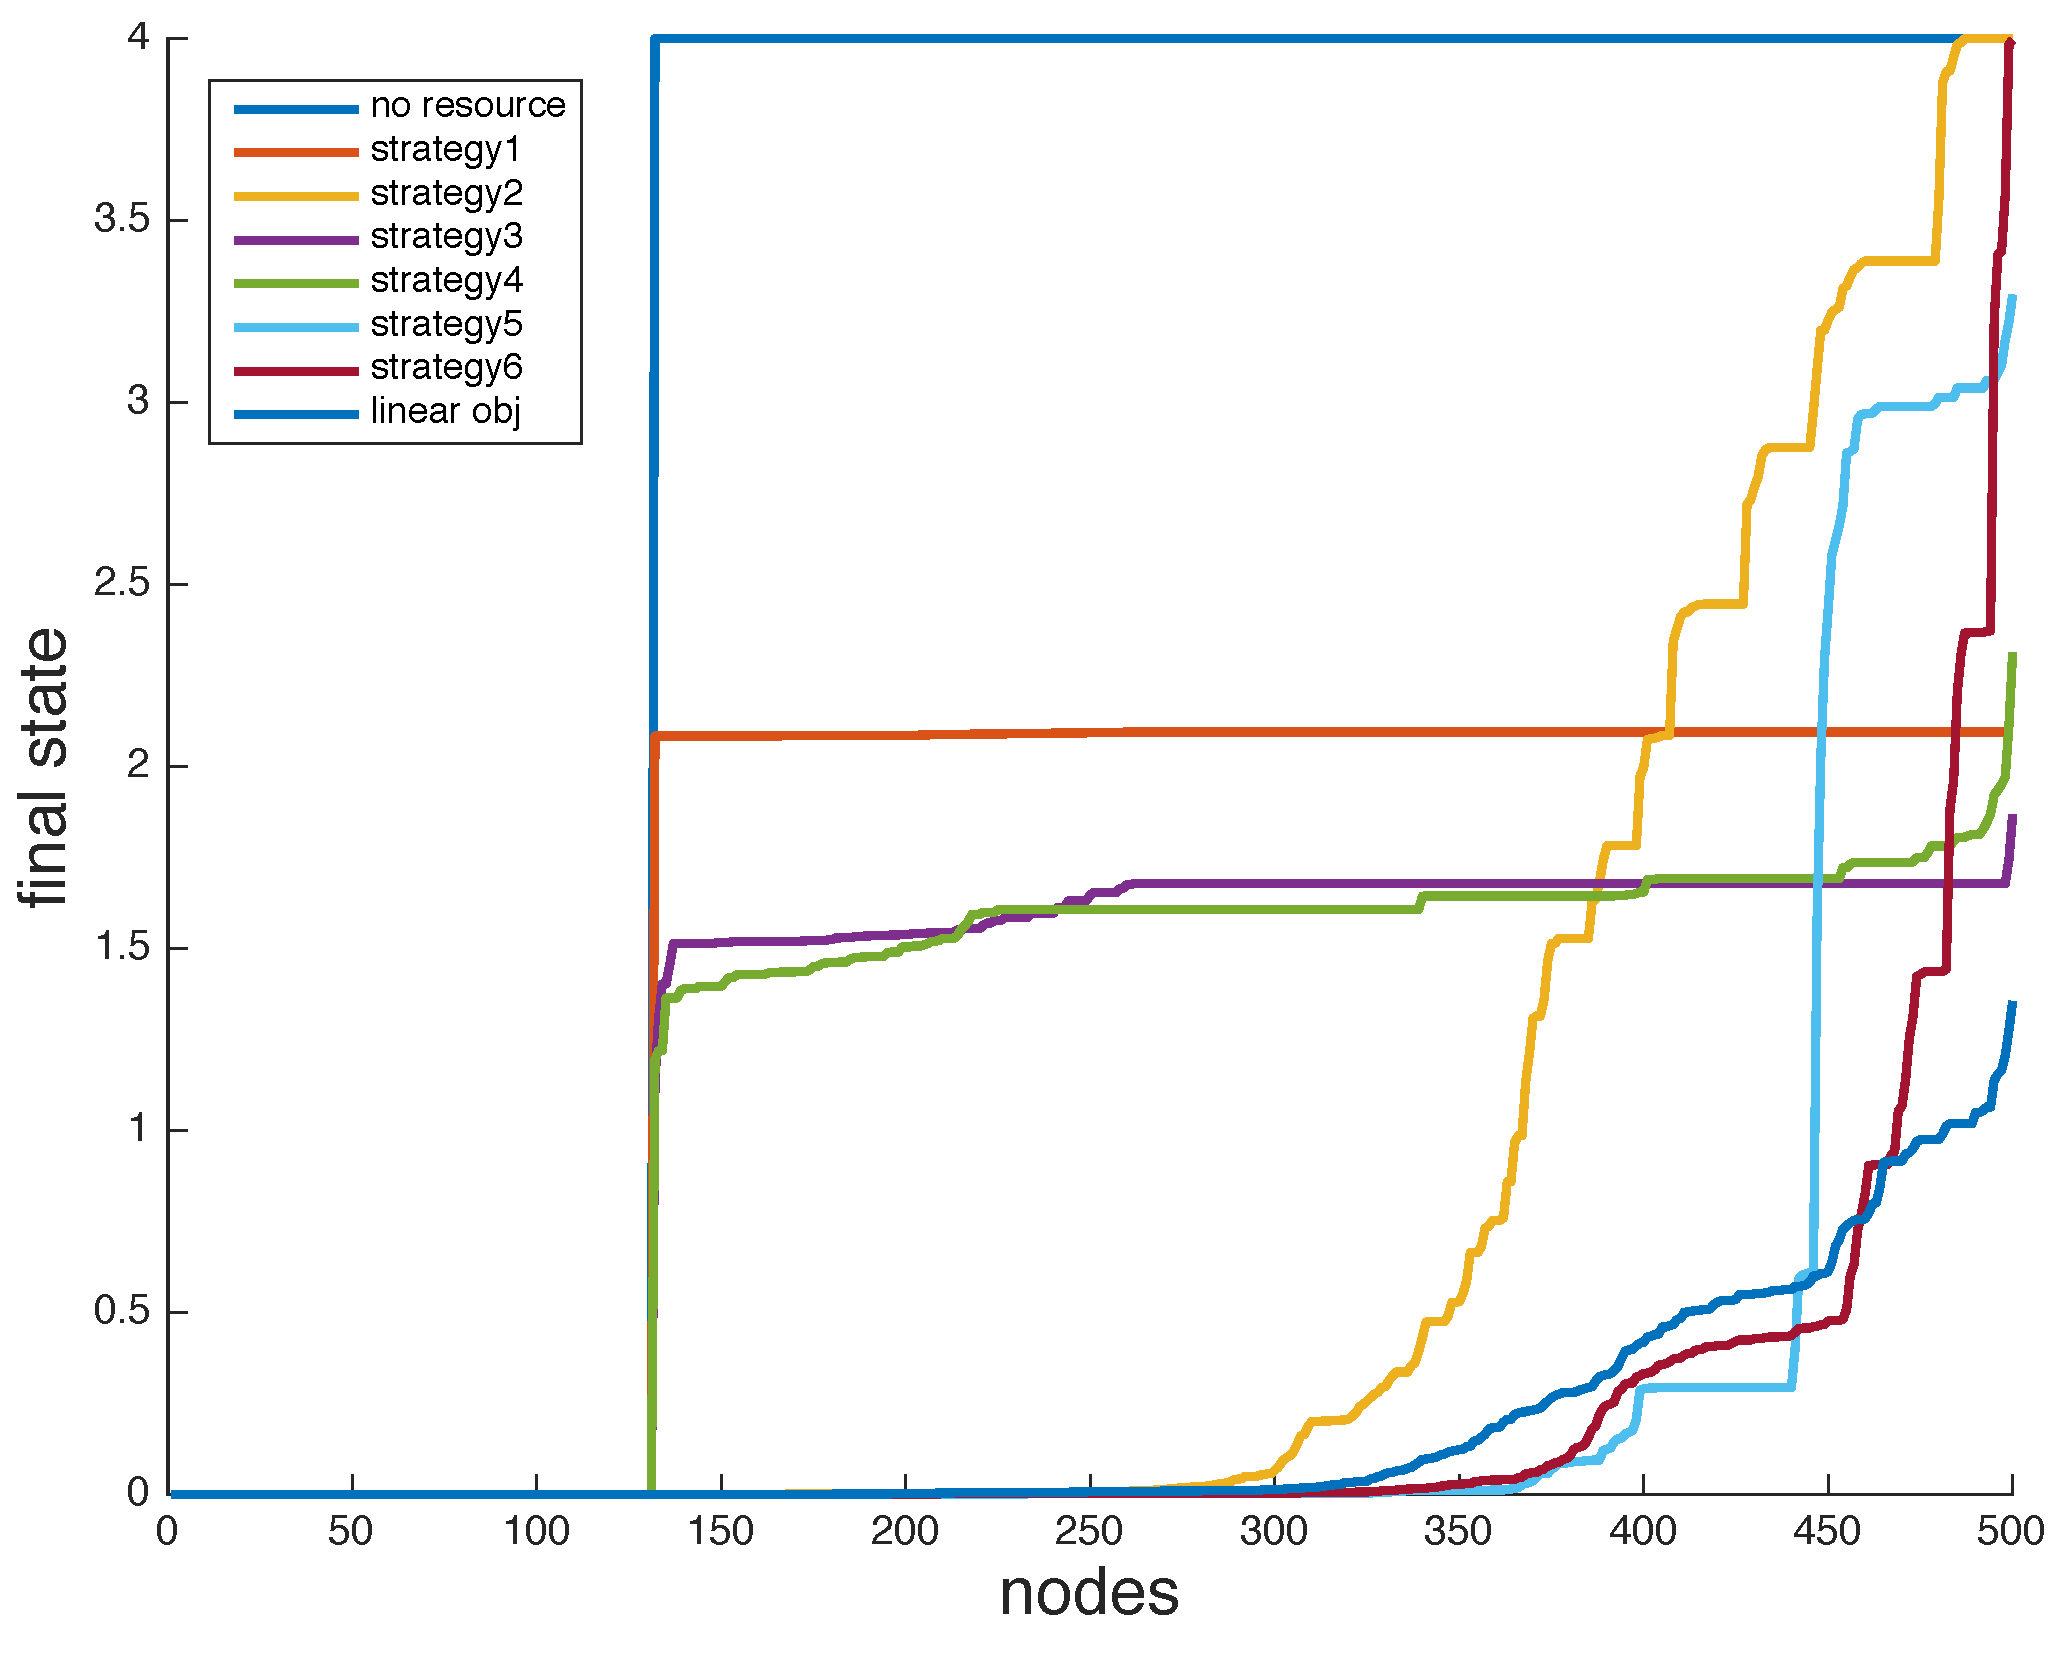
\includegraphics[height=80mm]{../figs/no_linear_approximation/SF_finalState_small.pdf}
		\caption{Final states on scale-free network}
	\end{subfigure}
	\caption{(a) Number of damaged nodes and (b) final states on grid network. Parameter setting is the same with that in grid network except for total external resources, i.e. $t_D=8$ and maximal iterations of gradient descent is 100. Because \textbf{S6} has achieve best result with 1000 external resources, in order to discriminate these strategies we decrease external resources to 600.}
	\label{fig:opt_on_sf}
\end{figure}





